\subsection{Shared Data and Data Hazards}

\begin{frame}[fragile]{Example: Data Hazards in Summation}
\begin{minted}[fontsize=\scriptsize]{c}
#include <stdio.h>
#include "omp.h"
int main() {
    int a[100];
    int sum = 0;
    // initialize
    for (int i = 0; i < 100; i++) a[i] = i + 1;
    // Sum up from 1 to 100
#pragma omp parallel for
    for (int i = 0; i < 100; i++) {
        sum += a[i];
    }
    printf("Sum = %d\n", sum);
}
\end{minted}
\end{frame}

\begin{frame}[fragile]{How Data Hazards Happen?}
\begin{columns}[T]
    \begin{column}{0.7\textwidth}
        \begin{figure}
            \centering
            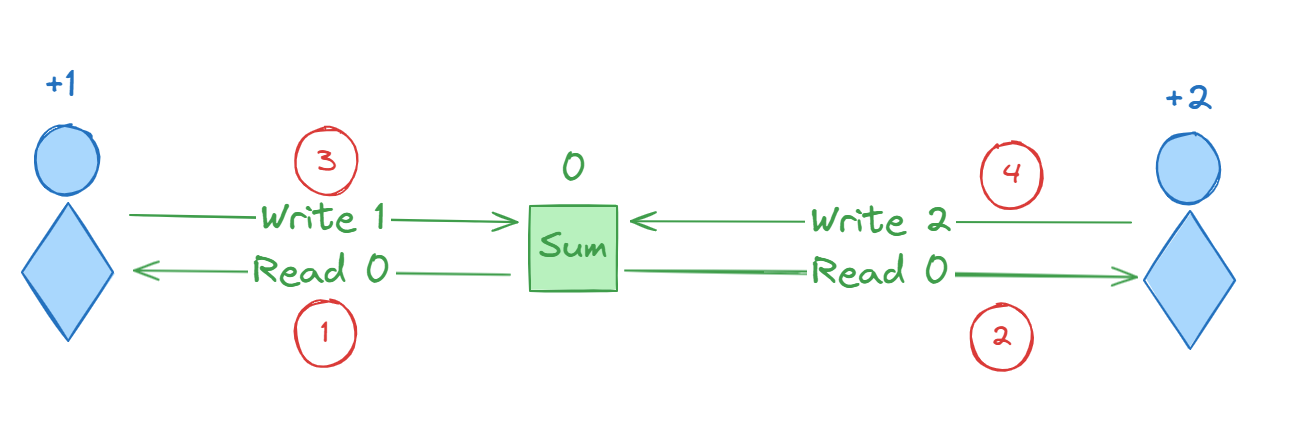
\includegraphics[width=\textwidth]{day8_am/img/hazard_illustration.png}
        \end{figure}
    \end{column}
    \begin{column}{0.3\textwidth}
        \begin{figure}
            \centering
            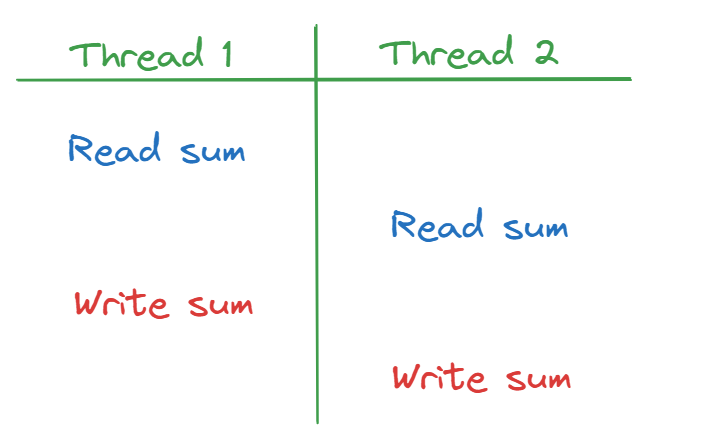
\includegraphics[width=\textwidth]{day8_am/img/hazard_schedule.png}
        \end{figure}
    \end{column}
\end{columns}
\end{frame}

\begin{frame}[fragile]{Scope and Data Hazard}
\begin{columns}[T]
    \begin{column}{0.5\textwidth}
        \begin{itemize}
            \item Shared \& private data in default
            \item Explicit scopes definition
            \begin{itemize}
                \item \textit{private}
                \item \textit{shared}
                \item \textit{firstprivate}
                \item \textit{lastprivate}
            \end{itemize}
            \item Data hazards happen when operating shared data
        \end{itemize}
    \end{column}
    \begin{column}{0.5\textwidth}
        \begin{minted}[fontsize=\scriptsize]{c}
    int sum = 0;
    // Sum up from 1 to 100
#pragma omp parallel for
    for (int i = 0; i <= 99; i++) {
        sum += a[i];
    }
\end{minted}
    \end{column}
\end{columns}
\end{frame}

\begin{frame}[fragile]{Resolve Data Hazard}
\begin{itemize}
    \item Critical Section
    \item Atomic Operations
    \item Reduction
\end{itemize}
\end{frame}

\begin{frame}[fragile]{Example: Solution with Critical Section}
\begin{columns}[T]
    \begin{column}{0.5\textwidth}
        \begin{itemize}
            \item Only one thread can enter critical section at the same time.
            \item A critical section can contain multiple statements.
        \end{itemize}
    \end{column}
    \begin{column}{0.5\textwidth}
\begin{minted}[fontsize=\scriptsize]{c}
#pragma omp parallel for
    for (int i = 0; i < 100; i++) {
#pragma omp critical
        { sum += a[i]; }
    }
    printf("Sum = %d\n", sum);
\end{minted}
    \end{column}
\end{columns}

\end{frame}

\begin{frame}[fragile]{Example: Solution with Atomic Operation}
\begin{columns}[T]
    \begin{column}{0.5\textwidth}
        \begin{itemize}
            \item Atomic operation cannot be separated.
            \item Only can be applied to one operation
            \item Limited set of operators supported
        \end{itemize}
    \end{column}
    \begin{column}{0.5\textwidth}
\begin{minted}[fontsize=\scriptsize]{c}
#pragma omp parallel for
    for (int i = 0; i < 100; i++) {
#pragma omp atomic
        sum += a[i];
    }
    printf("Sum = %d\n", sum);
\end{minted}
    \end{column}
\end{columns}
\end{frame}

\begin{frame}[fragile]{Example: Solution with Reduction}
\begin{columns}[T]
    \begin{column}{0.45\textwidth}
        \begin{itemize}
            \item Create temporary private variables for each thread
            \item Reduce these private variables in the end
            \item Limited set of operators supported
        \end{itemize}
    \end{column}
    \begin{column}{0.55\textwidth}
\begin{minted}[fontsize=\scriptsize]{c}
#pragma omp parallel for reduction(+:sum)
    for (int i = 0; i < 100; i++) {
        sum += a[i];
    }
    printf("Sum = %d\n", sum);
\end{minted}
    \end{column}
\end{columns}
\end{frame}

\begin{frame}[fragile]{Comparison}
\begin{itemize}
    \item Critical Region: Based on locking
    \item Atomic Operation: Based on hardware atomic operations
    \item Reduction: only synchronize in the end

\end{itemize}
\end{frame}

\begin{frame}[fragile]{Another Example: GEMM}
    \begin{minted}[fontsize=\scriptsize]{c}
    // General Matrix Multiplication (GEMM)
    for (int i = 0; i < N; i++) {
        for (int j = 0; j < N; j++) {
            c[i][j] = 0;
            for (int k = 0; k < N; k++) {
                c[i][j] += a[i][k] * b[k][j];
            }
        }
    }
    \end{minted}
\end{frame}

\begin{frame}[fragile]{Another Example: GEMM}
    \begin{minted}[fontsize=\scriptsize]{c}
#pragma omp parallel for collapse(3) reduction(+ : c)
    for (int i = 0; i < N; i++) {
        for (int j = 0; j < N; j++) {
            c[i][j] = 0;
            for (int k = 0; k < N; k++) {
                c[i][j] += a[i][k] * b[k][j];
            }
        }
    }
    \end{minted}
\end{frame}